% Provenance (never printed): cycle 3 / 6e "La planete Terre" (water in the
% ground, groundwater, springs and wells; resource); see
% sources/book1/PROVENANCE.md. Book 1, grade 6, chapter 5.
% Vocabulary guard: "sediment" not before g7.4; the water cycle is recalled
% from the physics book (prose only).
\chapter{Water Underground}\label{ch:g6:water-underground}

On a hot summer day, the fields are dry and the streams are low. Yet at the
foot of a \omterm{def:g1:landscapes-around-us:landform}{hill}, water keeps rising out of the ground, cold and clear, as it
did all winter, and fills a pool. It has not rained for weeks. Where does
this water come from, and how does it get out of the \omterm{def:g3:stones-pebbles-sand:rock}{rock}?

\begin{omfigure}
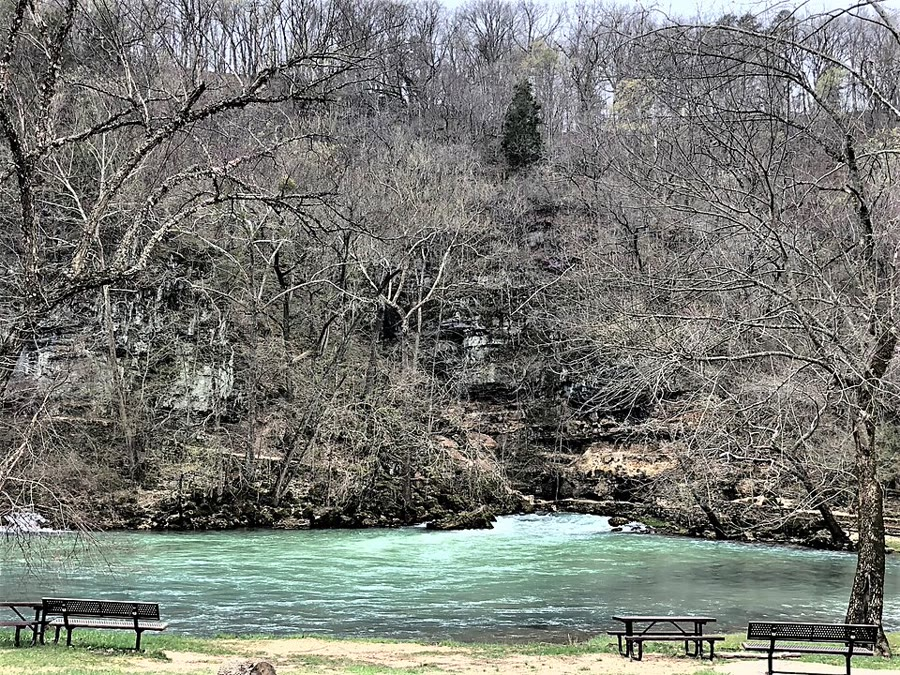
\includegraphics[width=0.72\linewidth]{images/book1/g6-big-spring.jpg}

{\small A \omterm{def:g6:water-underground:spring}{spring} rises at the foot of a rocky bluff and fills a pool: Big
Spring, Missouri (United States). (Photo: Johnston9494, CC BY-SA 4.0, via
Wikimedia Commons.)}
% ledger: commons:big-spring
\end{omfigure}

\begin{recall}
Almost all the water on the Earth is \omterm{def:g2:water-on-earth:salt-fresh}{salt water}; \omterm{def:g2:water-on-earth:salt-fresh}{fresh water} is a small
part, kept mostly as ice and under the ground
(\cref{ch:g2:water-on-earth}). \omterm{def:g3:stones-pebbles-sand:rock}{Rocks} such as sandstone and limestone are
made of grains or shells stuck together, while clay and shale are made of
very fine particles (\cref{ch:g6:rocks-and-minerals}). In the physics book,
you have followed water around the water cycle: it evaporates from the
\omterm{def:g2:water-on-earth:ocean}{seas}, condenses into \omterm{def:g4:clouds-rain-snow:cloud}{clouds} and falls back as \omterm{def:g4:clouds-rain-snow:precipitation}{rain} or \omterm{def:g4:clouds-rain-snow:precipitation}{snow}.
\end{recall}

\section{Rain soaks in}

When \omterm{def:g4:clouds-rain-snow:precipitation}{rain} falls on the land, the water can take three paths. Part of it
evaporates back into the air. Part of it flows over the surface, down the
slopes, into streams and \omterm{def:g1:landscapes-around-us:water}{rivers}: this is \emph{run-off}. The rest soaks
into the ground.

\begin{definition}[Infiltration]\label{def:g6:water-underground:infiltration}
\emph{Infiltration}\index{infiltration} is the soaking of \omterm{def:g4:clouds-rain-snow:precipitation}{rain} water, or
melted \omterm{def:g4:clouds-rain-snow:precipitation}{snow}, into the ground, through the soil and down into the \omterm{def:g3:stones-pebbles-sand:rock}{rocks}.
\end{definition}

How much water soaks in depends on the ground. On a steep slope, on bare
or hard ground, on a road or a car park, or when the soil is already
soaked, most of the water runs off. On a gentle slope, under grass and
trees, on sandy soil, more of it has time to soak in.

\begin{omfigure}
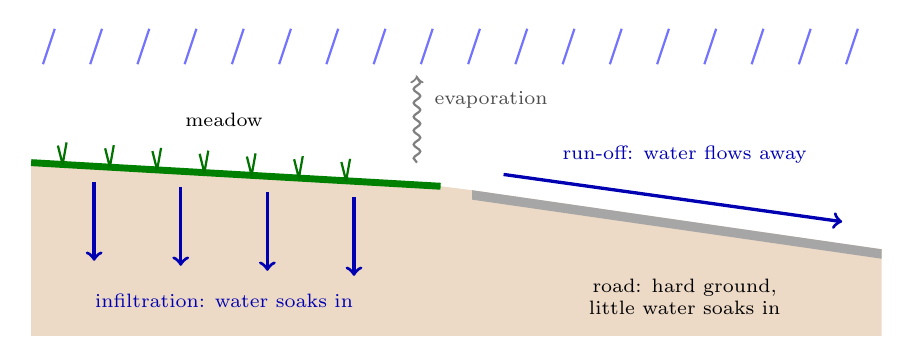
\begin{tikzpicture}[x=1cm, y=1cm]
  % rain
  \foreach \x in {0.3,0.9,...,10.5} \draw[blue!55, thick] (\x,3.9) -- (\x-0.15,3.45);
  % ground: field on the left (gentle), road and town on the right
  \fill[brown!30] (0,0) -- (0,2.2) -- (5.2,1.9) -- (5.6,1.85) -- (10.8,1.1) -- (10.8,0) -- cycle;
  \draw[green!50!black, line width=2.5pt] (0,2.2) -- (5.2,1.9);
  \fill[gray!70] (5.6,1.85) -- (10.8,1.1) -- (10.8,0.98) -- (5.6,1.73) -- cycle;
  \foreach \x in {0.4,1.0,...,4.6} \draw[green!45!black, thick] (\x,{2.2-0.058*\x}) -- ++(0.05,0.28) (\x,{2.2-0.058*\x}) -- ++(-0.06,0.24);
  % infiltration arrows in the field
  \foreach \x in {0.8,1.9,3.0,4.1} \draw[->, blue!70!black, very thick] (\x,{2.0-0.058*\x}) -- ++(0,-1.0);
  \node[font=\scriptsize, blue!70!black, align=center, fill=brown!30] at (2.45,0.45) {infiltration: water soaks in};
  % run-off on the road
  \draw[->, blue!70!black, very thick] (6.0,2.05) -- (10.3,1.45);
  \node[font=\scriptsize, blue!70!black, align=center] at (8.3,2.3) {run-off: water flows away};
  \node[font=\scriptsize, align=center] at (8.3,0.5) {road: hard ground,\\ little water soaks in};
  \node[font=\scriptsize] at (2.45,2.75) {meadow};
  % evaporation
  \draw[->, gray, thick, decorate, decoration={snake, amplitude=1.2pt, segment length=5pt}] (4.9,2.2) -- (4.9,3.3);
  \node[font=\scriptsize, gray!60!black, anchor=west] at (5.0,3.0) {evaporation};
\end{tikzpicture}

{\small The three paths of \omterm{def:g4:clouds-rain-snow:precipitation}{rain} water. In the meadow much of it soaks in;
on the road most of it runs off.}
\end{omfigure}

\section{Porous and permeable rocks}

Look at a handful of dry \omterm{def:g3:stones-pebbles-sand:sand}{sand} through a hand lens: between the grains there
are tiny empty spaces. Pour water on it and the water fills these spaces.
Many \omterm{def:g3:stones-pebbles-sand:rock}{rocks} are like that: they are full of small holes between their grains,
or of thin cracks.

\begin{definition}[Porosity]\label{def:g6:water-underground:porosity}
The \emph{pores}\index{pore} of a \omterm{def:g3:stones-pebbles-sand:rock}{rock} are the empty spaces between its grains
and in its cracks. A \omterm{def:g3:stones-pebbles-sand:rock}{rock} with pores is \emph{porous}\index{porous}. Its
\emph{porosity}\index{porosity} is the share of its volume made of pores,
written as a percentage.
\end{definition}

\begin{definition}[Permeability]\label{def:g6:water-underground:permeability}
A \omterm{def:g3:stones-pebbles-sand:rock}{rock} is \emph{permeable}\index{permeable} when water can flow through it,
because its \omterm{def:g6:water-underground:porosity}{pores} are large enough and connected to one another. It is
\emph{impermeable}\index{impermeable} when water cannot flow through it.
\emph{Permeability}\index{permeability} is how easily water flows through
a \omterm{def:g3:stones-pebbles-sand:rock}{rock}.
\end{definition}

The two ideas are not the same. Clay is very \omterm{def:g6:water-underground:porosity}{porous}: half of its volume is
made of \omterm{def:g6:water-underground:porosity}{pores}. But its \omterm{def:g6:water-underground:porosity}{pores} are so tiny that the water stays stuck in
them: clay is \emph{\omterm{def:g6:water-underground:permeability}{impermeable}}. \omterm{def:g3:stones-pebbles-sand:sand}{Sand} has fewer \omterm{def:g6:water-underground:porosity}{pores} than clay, but they
are wide and connected: \omterm{def:g3:stones-pebbles-sand:sand}{sand} is \emph{\omterm{def:g6:water-underground:permeability}{permeable}}. Granite without cracks
has almost no \omterm{def:g6:water-underground:porosity}{pores} at all.
% ledger: heath:porosity

\begin{omfigure}
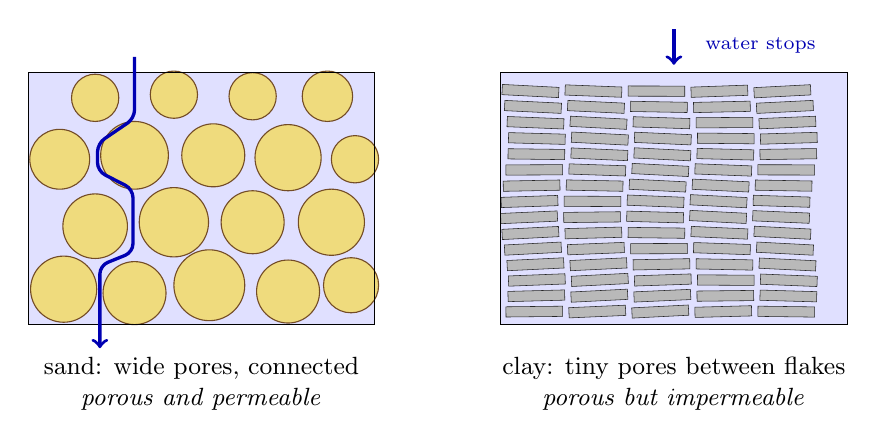
\begin{tikzpicture}
  % sand
  \begin{scope}
    \fill[blue!12] (0,0) rectangle (4.4,3.2);
    \foreach \x/\y/\r in {0.45/0.45/0.42, 1.35/0.4/0.4, 2.3/0.5/0.45, 3.3/0.42/0.4, 4.1/0.5/0.35,
                         0.85/1.25/0.41, 1.85/1.3/0.44, 2.85/1.3/0.4, 3.85/1.3/0.42,
                         0.4/2.1/0.38, 1.35/2.15/0.43, 2.35/2.15/0.4, 3.3/2.12/0.42, 4.15/2.1/0.3,
                         0.85/2.88/0.3, 1.85/2.92/0.3, 2.85/2.9/0.3, 3.8/2.9/0.32}
      \fill[yellow!55!brown!60, draw=brown!60!black] (\x,\y) circle (\r);
    \draw (0,0) rectangle (4.4,3.2);
    \draw[->, blue!70!black, very thick, rounded corners=3pt] (1.35,3.4) -- (1.35,2.62) -- (0.88,2.3) -- (0.88,1.95) -- (1.33,1.72) -- (1.33,0.92) -- (0.91,0.75) -- (0.91,-0.3);
    \node[font=\small, align=center] at (2.2,-0.75) {sand: wide pores, connected\\ \emph{porous and permeable}};
  \end{scope}
  % clay
  \begin{scope}[xshift=6.0cm]
    \fill[blue!12] (0,0) rectangle (4.4,3.2);
    \foreach \y in {0.1,0.3,...,3.0}
      \foreach \x in {0.05,0.85,...,3.7}
        \fill[gray!55, draw=gray!30!black, line width=0.2pt, rotate around={{3*sin(57*\x+91*\y)}:(\x+0.36,\y+0.06)}]
          ({\x+0.05*sin(200*\y)},\y) rectangle ++(0.72,0.13);
    \draw (0,0) rectangle (4.4,3.2);
    \draw[->, blue!70!black, very thick] (2.2,3.75) -- (2.2,3.3);
    \node[font=\scriptsize, blue!70!black] at (3.3,3.55) {water stops};
    \node[font=\small, align=center] at (2.2,-0.75) {clay: tiny pores between flakes\\ \emph{porous but impermeable}};
  \end{scope}
\end{tikzpicture}

{\small The \omterm{def:g6:water-underground:porosity}{pores} (in blue) between the grains of a \omterm{def:g3:stones-pebbles-sand:sand}{sand} and between the
flakes of a clay, much enlarged. Water finds a way through the \omterm{def:g3:stones-pebbles-sand:sand}{sand}; in
the clay, it stays stuck.}
\end{omfigure}

The table gives the \omterm{def:g6:water-underground:porosity}{porosity} of a few materials, and the share of water
that drains out of them by itself when they are full of water. The rest
stays stuck to the grains.

\begin{center}\small
\begin{tabular}{|l|c|c|}
\hline
\textbf{material} & \textbf{\omterm{def:g6:water-underground:porosity}{porosity} (\%)} & \textbf{water that drains out (\%)} \\
\hline
soil & 55 & 40 \\
clay & 50 & 2 \\
\omterm{def:g3:stones-pebbles-sand:sand}{sand} & 25 & 22 \\
\omterm{def:g3:stones-pebbles-sand:pebble}{gravel} & 20 & 19 \\
limestone & 20 & 18 \\
sandstone & 11 & 6 \\
granite & 0.1 & 0.09 \\
\hline
\end{tabular}
\end{center}
% ledger: heath:porosity

\begin{method}[How much water does a rock hold?]\label{met:g6:water-underground:volume}
\begin{enumerate}
  \item Find the volume of the \omterm{def:g3:stones-pebbles-sand:rock}{rock} (for a block: length $\times$ width
        $\times$ height).
  \item Multiply by the \omterm{def:g6:water-underground:porosity}{porosity} and divide by 100: this is the volume of
        the \omterm{def:g6:water-underground:porosity}{pores}, so the water the \omterm{def:g3:stones-pebbles-sand:rock}{rock} holds when it is full.
  \item For the water that drains out, use the second percentage in the
        same way. (1~cubic metre is 1000~litres.)
\end{enumerate}
\end{method}

\begin{example}[A cubic metre of sand]\label{ex:g6:water-underground:sand}
One cubic metre of \omterm{def:g3:stones-pebbles-sand:sand}{sand}, full of water, holds $1000 \times 25 \div 100 =
250$~litres of water in its \omterm{def:g6:water-underground:porosity}{pores}. Of these, $1000 \times 22 \div 100 = 220$
litres drain out by themselves; 30~litres stay stuck to the grains. One
cubic metre of clay holds twice as much water, 500~litres, but only
20~litres drain out.
% ledger: heath:porosity
\end{example}

\begin{inthelab}[Sand or clay? (in class, with the teacher)]
Two flowerpots with a hole at the bottom stand over two glasses. One is
filled with dry \omterm{def:g3:stones-pebbles-sand:sand}{sand}, the other with dry clay soil pressed down. The teacher
pours the same glass of water into each, at the same time. Through the
\omterm{def:g3:stones-pebbles-sand:sand}{sand}, water soon drips into the glass below. On the clay, the water stays
on top as a puddle and only a few drops come through, slowly: the \omterm{def:g3:stones-pebbles-sand:sand}{sand} is
\omterm{def:g6:water-underground:permeability}{permeable}, the clay is not.
\end{inthelab}

\section{Groundwater and the water table}

Dig a hole in the \omterm{def:g3:stones-pebbles-sand:sand}{sand} of a beach, a few steps from the \omterm{def:g2:water-on-earth:ocean}{sea}: after a while,
water appears at the bottom of the hole. You have reached the place where
all the \omterm{def:g6:water-underground:porosity}{pores} of the \omterm{def:g3:stones-pebbles-sand:sand}{sand} are full of water.
% ledger: wss:aquifer

\begin{definition}[Groundwater]\label{def:g6:water-underground:groundwater}
\emph{Groundwater}\index{groundwater} is the water under the ground that
fills the \omterm{def:g6:water-underground:porosity}{pores} and cracks of the soil and of the \omterm{def:g3:stones-pebbles-sand:rock}{rocks}.
\end{definition}

\begin{definition}[Water table]\label{def:g6:water-underground:water-table}
Below a certain depth, all the \omterm{def:g6:water-underground:porosity}{pores} of the \omterm{def:g3:stones-pebbles-sand:rock}{rock} are full of water. The
\emph{water table}\index{water table} is the top of this water-filled zone.
Above it, the \omterm{def:g6:water-underground:porosity}{pores} hold air and a little water; below it, they are full of
water.
% ledger: wss:aquifer
\end{definition}

The \omterm{def:g6:water-underground:water-table}{water table} is not flat. It follows the shape of the land, but more
gently: higher under the \omterm{def:g1:landscapes-around-us:landform}{hills}, lower under the \omterm{def:g1:landscapes-around-us:landform}{valleys}. It also moves up
and down with the seasons. After a rainy season, the \omterm{def:g4:clouds-rain-snow:precipitation}{rain} that has soaked
in raises it; after a long dry season, the water slowly flows away to
\omterm{def:g6:water-underground:spring}{springs} and \omterm{def:g1:landscapes-around-us:water}{rivers}, and the \omterm{def:g6:water-underground:water-table}{water table} goes down.

\omterm{def:g6:water-underground:groundwater}{Groundwater} is a great store of \omterm{def:g2:water-on-earth:salt-fresh}{fresh water}. Of all the \omterm{def:g2:water-on-earth:salt-fresh}{fresh water} of the
Earth, about 69~\% is ice and permanent \omterm{def:g4:clouds-rain-snow:precipitation}{snow}, and about 30~\% is
\omterm{def:g6:water-underground:groundwater}{groundwater}; the \omterm{def:g2:water-on-earth:salt-fresh}{fresh water} of all the \omterm{def:g1:landscapes-around-us:water}{lakes} makes only about a quarter
of one percent. \omterm{def:g6:water-underground:groundwater}{Groundwater} is more than a hundred times as abundant as
the \omterm{def:g2:water-on-earth:salt-fresh}{fresh water} of the \omterm{def:g1:landscapes-around-us:water}{lakes}.
% ledger: wss:fresh-shares

\begin{omfigure}
\begin{tikzpicture}
  \begin{axis}[xbar, width=0.8\linewidth, height=3.9cm, bar width=8pt,
      xmin=0, xmax=85, ymin=-0.6, ymax=4.6, y dir=reverse,
      ytick={0,...,4}, yticklabels from table={figdata/out/grade-6-water_table-fresh.dat}{label},
      xlabel={percent of all the fresh water of the Earth},
      axis x line=bottom, axis y line=left, axis line style={-},
      tick label style={font=\scriptsize}, label style={font=\small},
      nodes near coords, nodes near coords style={font=\scriptsize, anchor=west},
      point meta=explicit symbolic, enlarge y limits=false, clip=false]
    \addplot[fill=blue!35, draw=blue!60!black] table[x=pct, y=idx, meta=pct] {figdata/out/grade-6-water_table-fresh.dat};
  \end{axis}
\end{tikzpicture}

{\small Where the Earth's \omterm{def:g2:water-on-earth:salt-fresh}{fresh water} is. The bars for the \omterm{def:g1:landscapes-around-us:water}{lakes} and for
everything else (\omterm{def:g1:landscapes-around-us:water}{rivers}, the air, the soil, swamps, living things) are too
short to see.}
% ledger: wss:fresh-shares (figdata/grade-6/water_table.py, part fresh)
\end{omfigure}

\section{Springs and wells}

\begin{definition}[Spring and well]\label{def:g6:water-underground:spring}
A \emph{spring}\index{spring} is a place where \omterm{def:g6:water-underground:groundwater}{groundwater} comes out of the
ground by itself, where the \omterm{def:g6:water-underground:water-table}{water table} meets the surface. A
\emph{well}\index{well} is a hole dug or drilled down below the \omterm{def:g6:water-underground:water-table}{water
table}, so that \omterm{def:g6:water-underground:groundwater}{groundwater} fills its bottom and can be lifted out.
\end{definition}

The section below crosses a \omterm{def:g1:landscapes-around-us:landform}{valley} of the Varden Hills, the region of our
exercises. The \omterm{def:g1:landscapes-around-us:landform}{hills} are made of chalk, a white, soft, \omterm{def:g6:water-underground:porosity}{porous} and \omterm{def:g6:water-underground:permeability}{permeable}
limestone. Under the chalk lies a layer of shale, which is \omterm{def:g6:water-underground:permeability}{impermeable}.
\omterm{def:g4:clouds-rain-snow:precipitation}{Rain} soaks into the chalk, fills its \omterm{def:g6:water-underground:porosity}{pores} and stops on the shale.

\begin{omfigure}
\begin{tikzpicture}
\begin{axis}[omsection, width=0.95\linewidth, height=7.2cm,
    xmin=0, xmax=2.8, ymin=0, ymax=560,
    xlabel={distance from the south end of the section (km)},
    ylabel={height above sea level (m)},
    tick label style={font=\scriptsize}, label style={font=\small},
    clip mode=individual]
  \addplot[om lith={icsJurassic!40}{om limestone}, draw=black, line width=0.3pt, even odd rule] table {figdata/out/grade-6-water_table-unit-limestone.dat};
  \addplot[om lith={icsJurassic!15}{om shale}, draw=black, line width=0.3pt, even odd rule] table {figdata/out/grade-6-water_table-unit-shale.dat};
  \addplot[om lith={icsCretaceous!35}{om limestone}, draw=black, line width=0.3pt, even odd rule] table {figdata/out/grade-6-water_table-unit-chalk.dat};
  \addplot[lith alluvium, draw=black, line width=0.3pt, even odd rule] table {figdata/out/grade-6-water_table-unit-alluvium.dat};
  \addplot[black, thick] table {figdata/out/grade-6-water_table-ground.dat};
  \addplot[blue!75!black, very thick] table {figdata/out/grade-6-water_table-wet.dat};
  \addplot[blue!75!black, very thick, dashed] table {figdata/out/grade-6-water_table-dry.dat};
  % wells
  \addplot[fill=white, draw=black, line width=0.4pt] table {figdata/out/grade-6-water_table-well-rects.dat};
  \addplot[only marks, mark=none, point meta=explicit symbolic, nodes near coords,
    nodes near coords style={font=\scriptsize\bfseries, anchor=south east, fill=white, fill opacity=0.8, text opacity=1, inner sep=1pt}]
    table[x=s_km, y=z_m, meta=label] {figdata/out/grade-6-water_table-well-labels.dat};
  % river and spring
  \addplot[only marks, mark=*, mark size=2.2pt, blue!75!black] table[x=s_km, y=z_m] {figdata/out/grade-6-water_table-points.dat};
  \node[font=\scriptsize, blue!70!black, anchor=south east] at (axis cs:0.215,140) {river};
  \node[font=\scriptsize, blue!70!black, anchor=east] at (axis cs:0.83,218) {spring};
  \node[font=\scriptsize] at (axis cs:2.2,470) {chalk (permeable)};
  \node[font=\scriptsize, fill=white, fill opacity=0.8, text opacity=1] at (axis cs:2.2,95) {shale (impermeable)};
  \node[font=\scriptsize, fill=white, fill opacity=0.8, text opacity=1] at (axis cs:0.95,25) {limestone};
  \node[font=\scriptsize, blue!70!black, fill=white, fill opacity=0.8, text opacity=1, align=center] at (axis cs:2.15,250) {water table:\\ after the rainy season (solid)\\ after the dry season (dashed)};
\end{axis}
\end{tikzpicture}

{\small A north--south section through the Varden Hills, from the \omterm{def:g1:landscapes-around-us:water}{river} up
the northern hillside (heights exaggerated about 2~times). The water held in
the chalk stops on the shale and comes out as a \omterm{def:g6:water-underground:spring}{spring} where the base of
the chalk meets the slope. \omterm{def:g6:water-underground:spring}{Well}~A always reaches the water; \omterm{def:g6:water-underground:spring}{well}~B reaches
it only after the rainy season.}
% (figdata/grade-6/water_table.py; region model figdata/shared/region.py)
\end{omfigure}

The \omterm{def:g6:water-underground:spring}{spring} flows where the base of the chalk meets the hillside: the water
cannot go down through the shale, so it flows along the top of the shale
and comes out on the slope. As long as there is water in the chalk above
the shale, the \omterm{def:g6:water-underground:spring}{spring} keeps running, even in a dry summer: that is the
answer to the question asked at the start of the chapter.

Look at the two \omterm{def:g6:water-underground:spring}{wells}. \omterm{def:g6:water-underground:spring}{Well}~A is 100~m deep; its bottom is below the \omterm{def:g6:water-underground:water-table}{water
table} in every season, so it always gives water. \omterm{def:g6:water-underground:spring}{Well}~B is even deeper,
105~m, but it was dug higher up the \omterm{def:g1:landscapes-around-us:landform}{hill}: its bottom is below the \omterm{def:g6:water-underground:water-table}{water
table} after the rainy season and above it after the dry season. In summer,
\omterm{def:g6:water-underground:spring}{well}~B runs dry. What matters is not how deep a \omterm{def:g6:water-underground:spring}{well} is, but how far its
bottom goes below the lowest \omterm{def:g6:water-underground:water-table}{water table}.
% (figdata/grade-6/water_table.py, part wells)

\begin{omfigure}
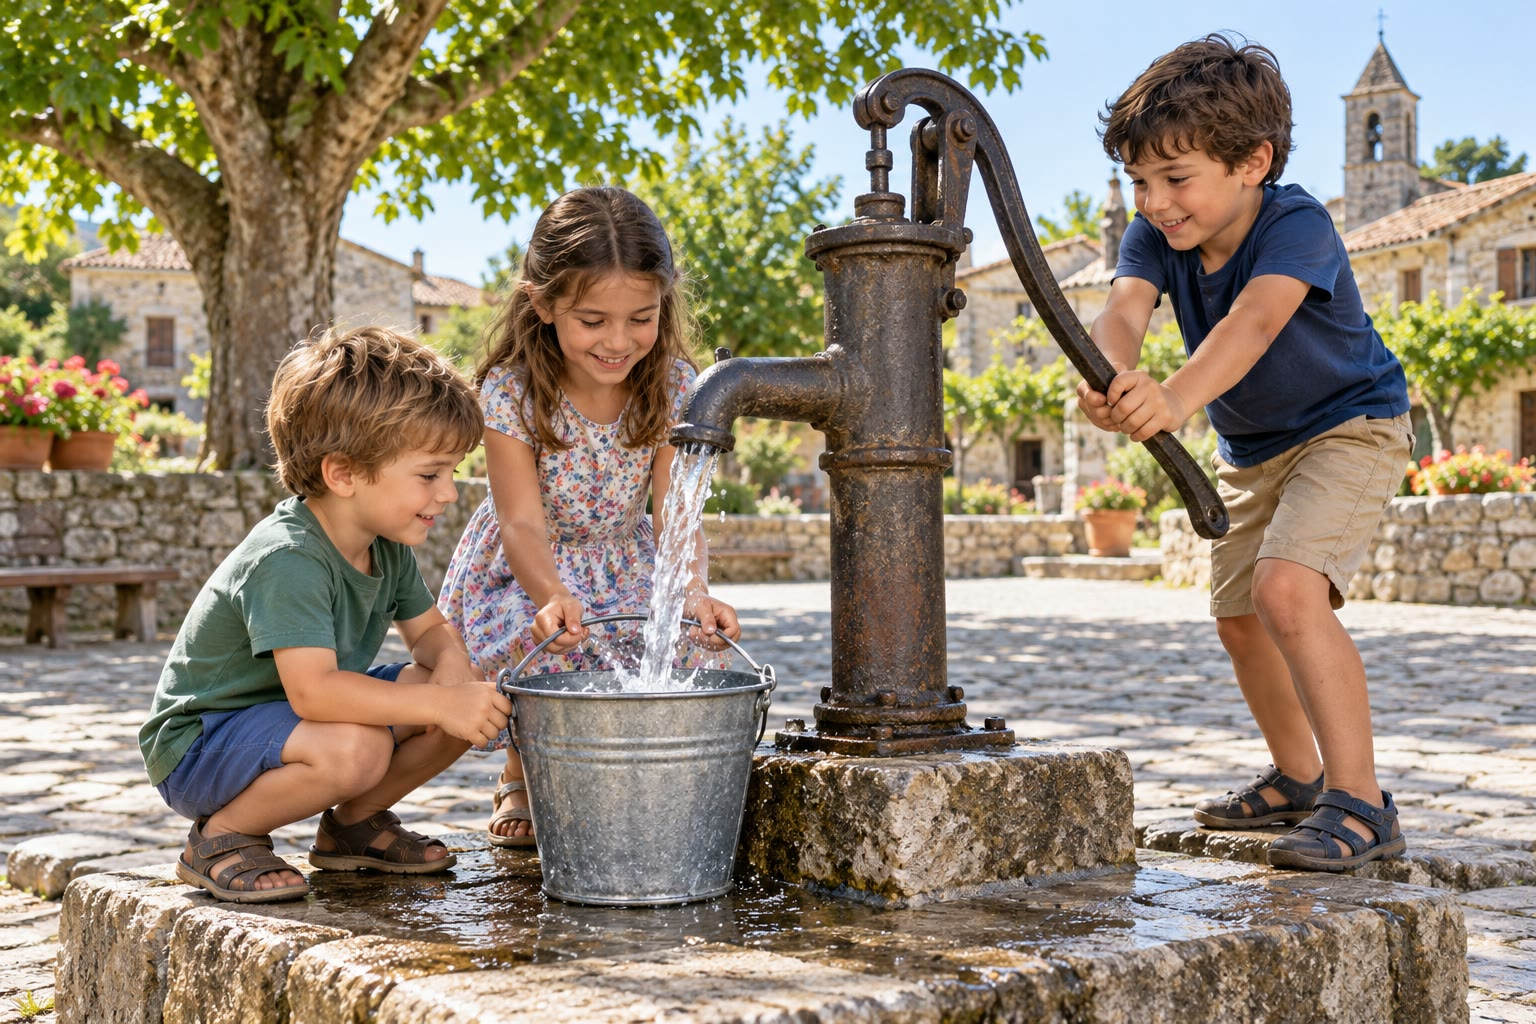
\includegraphics[width=0.6\linewidth]{images/book1/ai/g6-hand-pump.jpg}

{\small Children fill a bucket at the hand pump of a village \omterm{def:g6:water-underground:spring}{well}. (AI
illustration.)}
\end{omfigure}

\begin{remark}[A well can run dry]\label{rem:g6:water-underground:pumping}
Pumping water out of a \omterm{def:g6:water-underground:spring}{well} lowers the \omterm{def:g6:water-underground:water-table}{water table} around it. If water is
pumped out faster than the \omterm{def:g4:clouds-rain-snow:precipitation}{rain} refills the \omterm{def:g3:stones-pebbles-sand:rock}{rock}, the \omterm{def:g6:water-underground:water-table}{water table} goes down
and down: the \omterm{def:g6:water-underground:spring}{well} gives less and less water and can run dry. Two
neighbours pumping from the same \omterm{def:g3:stones-pebbles-sand:rock}{rock} share the same water: one pump can
dry out the other's \omterm{def:g6:water-underground:spring}{well}.
% ledger: wss:aquifer
\end{remark}

\section{Aquifers}

\begin{definition}[Aquifer]\label{def:g6:water-underground:aquifer}
An \emph{aquifer}\index{aquifer} is a layer of \omterm{def:g6:water-underground:porosity}{porous} and \omterm{def:g6:water-underground:permeability}{permeable} \omterm{def:g3:stones-pebbles-sand:rock}{rock},
full of \omterm{def:g6:water-underground:groundwater}{groundwater}, that lets this water flow out to \omterm{def:g6:water-underground:spring}{springs} and \omterm{def:g6:water-underground:spring}{wells}.
The \omterm{def:g4:clouds-rain-snow:precipitation}{rain} that soaks in refills it.
% ledger: wss:aquifer
\end{definition}

The chalk of the Varden Hills is an \omterm{def:g6:water-underground:aquifer}{aquifer}: it is \omterm{def:g6:water-underground:porosity}{porous}, it is \omterm{def:g6:water-underground:permeability}{permeable},
and the farms of the \omterm{def:g1:landscapes-around-us:landform}{hills} draw their water from it. The shale under it is
not an \omterm{def:g6:water-underground:aquifer}{aquifer}: water cannot flow through it. Deeper still, under the
shale, lie a limestone and a sandstone, which can hold water too; to reach
it, a \omterm{def:g6:water-underground:spring}{well} has to be drilled right through the shale.

\omterm{def:g6:water-underground:groundwater}{Groundwater} is part of the water cycle. \omterm{def:g4:clouds-rain-snow:precipitation}{Rain} soaks into an \omterm{def:g6:water-underground:aquifer}{aquifer};
\omterm{def:g6:water-underground:groundwater}{groundwater} flows slowly through the \omterm{def:g6:water-underground:porosity}{pores}; it comes out at \omterm{def:g6:water-underground:spring}{springs} and into \omterm{def:g1:landscapes-around-us:water}{rivers}, which carry it to the \omterm{def:g2:water-on-earth:ocean}{sea}; there
it evaporates, and falls again as \omterm{def:g4:clouds-rain-snow:precipitation}{rain}. Taking water from an \omterm{def:g6:water-underground:aquifer}{aquifer} is like
taking water from a tank that the \omterm{def:g4:clouds-rain-snow:precipitation}{rain} fills slowly: it lasts only if we do
not take more than the \omterm{def:g4:clouds-rain-snow:precipitation}{rain} brings back.

\section{Keeping groundwater clean}

Water that soaks into the ground is filtered on its way: leaves, soil
particles and small creatures are held back by the soil and the \omterm{def:g3:stones-pebbles-sand:rock}{rock}. That
is why water from a \omterm{def:g6:water-underground:spring}{spring} or a \omterm{def:g6:water-underground:spring}{well} usually looks crystal clear. But
substances \emph{dissolved} in the water are not held back: they travel
down with it to the \omterm{def:g6:water-underground:water-table}{water table}.
% ledger: wss:gw-quality

\omterm{def:g6:water-underground:groundwater}{Groundwater} can be spoilt by what people put on the ground: fertilisers and
pesticides spread on fields and gardens, salt spread on icy roads, fuel
leaking from a tank, waste dumped in the open, the overflow of badly kept
waste-water tanks of houses. Once dissolved in an \omterm{def:g6:water-underground:aquifer}{aquifer}, these substances
are hard to remove, and the water may no longer be safe to drink without
treatment. So the water of a \omterm{def:g6:water-underground:spring}{well} has to be tested before it is drunk, and fertilisers, fuel and waste are best kept far from \omterm{def:g6:water-underground:spring}{wells} and \omterm{def:g6:water-underground:spring}{springs}.
% ledger: wss:gw-quality

Dissolved substances travel with the \omterm{def:g6:water-underground:groundwater}{groundwater}. Below the \omterm{def:g6:water-underground:water-table}{water table},
the water creeps slowly downhill: from where the \omterm{def:g6:water-underground:water-table}{water table} is high, under
the \omterm{def:g1:landscapes-around-us:landform}{hills}, to where it is low, at the \omterm{def:g6:water-underground:spring}{springs} and the \omterm{def:g1:landscapes-around-us:water}{rivers}. A spill that
soaks in therefore does not stay where it fell. It sinks to the \omterm{def:g6:water-underground:water-table}{water
table}, then drifts downhill with the \omterm{def:g6:water-underground:groundwater}{groundwater}, towards whatever lies
below it on the slope.
% ledger: wss:gw-quality, wss:aquifer

\begin{omfigure}
\begin{tikzpicture}[x=1cm, y=1.15cm, font=\scriptsize]
  % ground (the chalk) and the water-filled zone under the water table
  \fill[black!6] (0,0) -- (0,4.090) -- plot[smooth] coordinates {(0.00,4.090) (1.00,4.013) (2.00,3.887) (3.00,3.692) (4.00,3.407) (5.00,3.033) (6.00,2.600) (7.00,2.167) (8.00,1.793) (9.00,1.508) (10.00,1.313) (11.00,1.187) (12.00,1.110)} -- (12,0) -- cycle;
  \fill[blue!14] (0,0) -- (0,3.190) -- plot[smooth] coordinates {(0.00,3.190) (1.00,3.185) (2.00,3.131) (3.00,3.008) (4.00,2.795) (5.00,2.493) (6.00,2.132) (7.00,1.771) (8.00,1.469) (9.00,1.256) (10.00,1.133) (11.00,1.079) (12.00,1.074)} -- (12,0) -- cycle;
  \draw[black!70, line width=0.7pt] plot[smooth] coordinates {(0.00,4.090) (1.00,4.013) (2.00,3.887) (3.00,3.692) (4.00,3.407) (5.00,3.033) (6.00,2.600) (7.00,2.167) (8.00,1.793) (9.00,1.508) (10.00,1.313) (11.00,1.187) (12.00,1.110)};
  \draw[blue!70!black, dashed, line width=0.7pt] plot[smooth] coordinates {(0.00,3.190) (1.00,3.185) (2.00,3.131) (3.00,3.008) (4.00,2.795) (5.00,2.493) (6.00,2.132) (7.00,1.771) (8.00,1.469) (9.00,1.256) (10.00,1.133) (11.00,1.079) (12.00,1.074)};
  % the spill: down to the water table, then downhill with the groundwater
  \fill[brown!70!black, opacity=0.55] (4.85,3.094) -- (5.15,2.971) -- (5.15,2.442) -- (4.85,2.544) -- cycle;
  \fill[brown!70!black, opacity=0.55] (4.85,2.514) -- (5.10,2.429) -- (5.35,2.341) -- (5.60,2.250) -- (5.85,2.158) -- (6.10,2.065) -- (6.35,1.972) -- (6.60,1.881) -- (6.85,1.792) -- (7.10,1.707) -- (7.35,1.626) -- (7.60,1.549) -- (7.85,1.478) -- (8.10,1.413) -- (8.35,1.354) -- (8.60,1.300) -- (8.85,1.252) -- (9.10,1.210) -- (9.30,1.181) -- (9.10,1.182) -- (8.85,1.190) -- (8.60,1.203) -- (8.35,1.221) -- (8.10,1.246) -- (7.85,1.277) -- (7.60,1.313) -- (7.35,1.355) -- (7.10,1.401) -- (6.85,1.486) -- (6.60,1.598) -- (6.35,1.713) -- (6.10,1.828) -- (5.85,1.945) -- (5.60,2.060) -- (5.35,2.174) -- (5.10,2.286) -- (4.85,2.394) -- cycle;
  % the leaking tank
  \draw[fill=black!35] (4.7,3.10) rectangle (5.3,3.42);
  \node[anchor=south, align=center] at (5.0,3.45) {leaking\\fuel tank};
  % groundwater flow
  \begin{scope}[blue!60!black, -{Stealth[length=2mm]}, line width=0.8pt]
    \draw (0.80,2.589) -- (2.40,2.491);
    \draw (3.40,2.334) -- (5.00,1.893);
    \draw (5.90,1.569) -- (7.50,1.009);
    \draw (8.80,0.691) -- (10.60,0.494);
  \end{scope}
  \node[blue!60!black, anchor=north] at (6.7,1.0) {groundwater flows downhill};
  % the two wells
  \draw[line width=1.6pt, black!75] (2.0,3.887) -- (2.0,2.70);
  \draw[line width=1.6pt, black!75] (8.5,1.639) -- (8.5,0.95);
  \node[anchor=south, align=center] at (2.0,3.95) {well A\\(uphill): clean};
  \draw[black!50] (8.5,1.66) -- (8.5,2.30);
  \node[anchor=south, align=center] at (8.5,2.30) {well B\\(downhill): spoilt};
  % the stream
  \fill[blue!60] (11.55,1.13) -- (11.95,1.11) -- (11.75,1.02) -- cycle;
  \node[anchor=south] at (11.6,1.20) {stream};
  \node[blue!70!black, anchor=south west] at (0.1,3.21) {water table};
  \node[anchor=west, black!70] at (0.15,0.25) {chalk};
\end{tikzpicture}

{\small A spill on a hillside (a sketch). The dissolved fuel sinks to the
\omterm{def:g6:water-underground:water-table}{water table}, then drifts downhill with the \omterm{def:g6:water-underground:groundwater}{groundwater} (blue arrows): it
reaches \omterm{def:g6:water-underground:spring}{well} B, below it on the slope, and in the end the stream. \omterm{def:g6:water-underground:spring}{Well} A,
uphill of the tank, stays clean.}
\end{omfigure}

\begin{method}[Is a well at risk?]\label{met:g6:water-underground:risk}
\begin{enumerate}
  \item Find where the \omterm{def:g6:water-underground:water-table}{water table} is high and where it is low: it is high
        under the \omterm{def:g1:landscapes-around-us:landform}{hills} and low near the \omterm{def:g6:water-underground:spring}{springs} and the \omterm{def:g1:landscapes-around-us:water}{rivers}.
  \item The \omterm{def:g6:water-underground:groundwater}{groundwater} flows from high to low: draw its direction with an
        arrow.
  \item A \omterm{def:g6:water-underground:spring}{well} or a \omterm{def:g6:water-underground:spring}{spring} that lies downhill of a source of pollution, on
        the path of that arrow, is at risk; a \omterm{def:g6:water-underground:spring}{well} uphill of it is not.
\end{enumerate}
\end{method}

\begin{example}[A new fuel tank for the farm]\label{ex:g6:water-underground:tank}
A farmer on a chalk hillside drinks the water of her own \omterm{def:g6:water-underground:spring}{well}, halfway up
the slope, and wants to put a new fuel tank in one of two fields: one
uphill of the \omterm{def:g6:water-underground:spring}{well}, one downhill of it, near the stream. The \omterm{def:g6:water-underground:groundwater}{groundwater}
flows downhill. A leak from the field uphill would drift down towards the
\omterm{def:g6:water-underground:spring}{well}; a leak from the field downhill would drift away from it, towards the
stream. The field downhill of the \omterm{def:g6:water-underground:spring}{well} is the better choice for the \omterm{def:g6:water-underground:spring}{well}
--- and a tank on a tray that holds any leak is better still, since the
stream matters too.
\end{example}

\begin{inthefield}[Spotting springs]
On a walk with an adult, look along the foot of a slope. A \omterm{def:g6:water-underground:spring}{spring} often
shows itself as a patch of wet ground, a line of greener grass or of reeds
in a dry field, a small stream that starts from nowhere, or a stone basin or
a trough built to catch the water. On a detailed walking \omterm{def:g2:drawing-to-map:map}{map}, \omterm{def:g6:water-underground:spring}{springs} are
marked with a small symbol. Observe from the path: never drink the
water of a \omterm{def:g6:water-underground:spring}{spring} that has not been tested.
\end{inthefield}

\section{Exercises}

\begin{exercise}[$\star$]\label{exo:g6:water-underground:1}
Sort these materials into ``\omterm{def:g6:water-underground:permeability}{permeable}'' and ``\omterm{def:g6:water-underground:permeability}{impermeable}'': \omterm{def:g3:stones-pebbles-sand:sand}{sand},
clay, \omterm{def:g3:stones-pebbles-sand:pebble}{gravel}, granite without cracks, shale, chalk.
\end{exercise}

\begin{exercise}[$\star$]\label{exo:g6:water-underground:2}
Match each word with its meaning: \omterm{def:g6:water-underground:spring}{spring}; \omterm{def:g6:water-underground:spring}{well}; \omterm{def:g6:water-underground:water-table}{water table}; \omterm{def:g6:water-underground:aquifer}{aquifer}.
(a) The top of the zone where all the \omterm{def:g6:water-underground:porosity}{pores} are full of water. (b) A
\omterm{def:g6:water-underground:porosity}{porous} and \omterm{def:g6:water-underground:permeability}{permeable} layer that holds \omterm{def:g6:water-underground:groundwater}{groundwater}. (c) A place where
\omterm{def:g6:water-underground:groundwater}{groundwater} comes out by itself. (d) A hole that goes down below the \omterm{def:g6:water-underground:water-table}{water
table}.
\end{exercise}

\begin{exercise}[$\star$]\label{exo:g6:water-underground:3}
(a) Name the three paths that \omterm{def:g4:clouds-rain-snow:precipitation}{rain} water can take when it falls on the
land. (b) After a \omterm{def:g5:natural-hazards:storm}{storm}, where does more water run off: on a car park or on
a meadow? Why?
\end{exercise}

\begin{exercise}[$\star$]\label{exo:g6:water-underground:4}
True or false? Correct the false sentences. (a) A \omterm{def:g6:water-underground:porosity}{porous} \omterm{def:g3:stones-pebbles-sand:rock}{rock} is always
\omterm{def:g6:water-underground:permeability}{permeable}. (b) Below the \omterm{def:g6:water-underground:water-table}{water table}, the \omterm{def:g6:water-underground:porosity}{pores} are full of water.
(c) The \omterm{def:g6:water-underground:water-table}{water table} is flat, like the surface of a \omterm{def:g1:landscapes-around-us:water}{lake}. (d) There is
more \omterm{def:g2:water-on-earth:salt-fresh}{fresh water} under the ground than in all the \omterm{def:g1:landscapes-around-us:water}{lakes}.
\end{exercise}

\begin{exercise}[$\star\star$]\label{exo:g6:water-underground:5}
A bucket holds 10~litres of dry \omterm{def:g3:stones-pebbles-sand:sand}{sand}. The \omterm{def:g6:water-underground:porosity}{porosity} of the \omterm{def:g3:stones-pebbles-sand:sand}{sand} is 25~\%.
How much water can you pour into the bucket before it overflows? How much
water would drain out through a hole in the bottom (22~\%)?
\end{exercise}

\begin{exercise}[$\star\star$]\label{exo:g6:water-underground:6}
A block of limestone measures 2~m by 1~m by 1~m. (a) What is its volume, in
cubic metres and in litres? (b) Its \omterm{def:g6:water-underground:porosity}{porosity} is 20~\%: how many litres of
water does it hold when it is full? (c) Of this water, 18~\% of the
volume drains out. How many litres drain out, and how many stay stuck?
\end{exercise}

\begin{exercise}[$\star\star$]\label{exo:g6:water-underground:7}
Use the section through the Varden Hills. (a) At what height is the \omterm{def:g6:water-underground:spring}{spring}?
the \omterm{def:g1:landscapes-around-us:water}{river}? (b) Is the \omterm{def:g6:water-underground:spring}{spring} above or below the \omterm{def:g1:landscapes-around-us:water}{river}? Where does the water
of the \omterm{def:g6:water-underground:spring}{spring} go? (c) Why is there no \omterm{def:g6:water-underground:spring}{spring} in the middle of the chalk
hillside?
\end{exercise}

\begin{exercise}[$\star\star$]\label{exo:g6:water-underground:8}
At \omterm{def:g6:water-underground:spring}{well}~A, the ground is at 401~m; the \omterm{def:g6:water-underground:water-table}{water table} is at 336~m after the
rainy season and at 314~m after the dry season. (a) How deep is the water
below the ground in each season? (b) By how many metres does the \omterm{def:g6:water-underground:water-table}{water table}
go down between the two seasons?
\end{exercise}

\begin{exercise}[$\star\star$]\label{exo:g6:water-underground:9}
A farmer wants a new \omterm{def:g6:water-underground:spring}{well} at the top of the \omterm{def:g1:landscapes-around-us:landform}{hill}, at the right end of the
section. Must the \omterm{def:g6:water-underground:spring}{well} be deeper or shallower than \omterm{def:g6:water-underground:spring}{well}~A? Explain with the
\omterm{def:g6:water-underground:water-table}{water table}.
\end{exercise}

\begin{exercise}[$\star\star$]\label{exo:g6:water-underground:10}
A cubic metre of clay holds 500~litres of water but gives only 20~litres.
Explain why a \omterm{def:g6:water-underground:spring}{well} dug into clay gives almost no water, although the clay
is full of it.
\end{exercise}

\begin{exercise}[$\star\star\star$]\label{exo:g6:water-underground:11}
Of all the \omterm{def:g2:water-on-earth:salt-fresh}{fresh water} of the Earth, 30.1~\% is \omterm{def:g6:water-underground:groundwater}{groundwater} and 0.26~\% is
in \omterm{def:g1:landscapes-around-us:water}{lakes}. (a) How many times more \omterm{def:g2:water-on-earth:salt-fresh}{fresh water} is there under the ground
than in the \omterm{def:g1:landscapes-around-us:water}{lakes}? (b) Of all \omterm{def:g2:water-on-earth:salt-fresh}{fresh water}, about 69~\% is ice and \omterm{def:g4:clouds-rain-snow:precipitation}{snow}.
What share is left for everything else (\omterm{def:g6:water-underground:groundwater}{groundwater}, \omterm{def:g1:landscapes-around-us:water}{lakes}, \omterm{def:g1:landscapes-around-us:water}{rivers}, the air,
the soil\ldots)? (c) Why is \omterm{def:g6:water-underground:groundwater}{groundwater} so important for drinking water?
\end{exercise}

\begin{exercise}[$\star\star\star$]\label{exo:g6:water-underground:12}
Two farms stand side by side on the same chalk. One summer, the first farm
installs a powerful pump and fills a large pond; a few weeks later, the
\omterm{def:g6:water-underground:spring}{well} of the second farm runs dry, although nobody touched it. Explain what
happened, and what the two farmers could do.
\end{exercise}

\section{Problem: The farm well of the Varden Hills}

\begin{problem}[{Weekend problem --- the rocks under a farm of the Varden
Hills, the water stored in its chalk, and how many days it would last
without rain}]
\label{pb:g6:water-underground:1}
% ledger: heath:porosity, wss:aquifer
A farm of the Varden Hills stands on the chalk, next to \omterm{def:g6:water-underground:spring}{well}~A of the
section. The farmer wants to know how long the \omterm{def:g6:water-underground:spring}{well} could keep the farm
going in a long \omterm{def:g5:natural-hazards:drought}{drought}, if no \omterm{def:g4:clouds-rain-snow:precipitation}{rain} at all came to refill the chalk.

\medskip
\noindent\textbf{Part I --- The rocks under the farm.}
\begin{enumerate}
  \item Name the \omterm{def:g3:stones-pebbles-sand:rock}{rock} on which the farm stands, and the \omterm{def:g3:stones-pebbles-sand:rock}{rock} under it. Which
        one is \omterm{def:g6:water-underground:permeability}{permeable}?
  \item Explain why a \omterm{def:g6:water-underground:spring}{spring} flows at the foot of the slope below the farm.
  \item Use the section: the ground at the farm is at 401~m and the \omterm{def:g6:water-underground:water-table}{water
        table} is at 336~m after the rainy season. How far down is the water?
  \item After the dry season, the \omterm{def:g6:water-underground:water-table}{water table} is at 314~m. \omterm{def:g6:water-underground:spring}{Well}~A is
        100~m deep. Does it still reach the water? By how many metres?
\end{enumerate}

\medskip
\noindent\textbf{Part II --- The water in the chalk.}
The farmer can drain the chalk around the \omterm{def:g6:water-underground:spring}{well} in a block 100~m long,
50~m wide and 2~m thick, below the \omterm{def:g6:water-underground:water-table}{water table}. The chalk is a limestone:
use a \omterm{def:g6:water-underground:porosity}{porosity} of 20~\% and a share of water that drains out of 18~\%.
\begin{enumerate}[resume]
  \item What is the volume of the block, in cubic metres?
  \item How many cubic metres of water fill its \omterm{def:g6:water-underground:porosity}{pores}?
  \item How many cubic metres of water drain out of it into the \omterm{def:g6:water-underground:spring}{well}? How
        many stay stuck in the chalk?
  \item Write the water that drains out in litres.
\end{enumerate}

\medskip
\noindent\textbf{Part III --- How long it lasts.}
\begin{enumerate}[resume]
  \item The farm (house, animals and vegetable garden) uses 18~cubic metres
        of water a day. How many litres is that?
  \item How much water does the farm use in a week?
  \item Why does the store of water in the chalk not run out in a normal
        year?
  \item Without any \omterm{def:g4:clouds-rain-snow:precipitation}{rain} at all, for how many days would the water draining
        out of the block supply the farm?
\end{enumerate}
\end{problem}
